\subsubsection{Admin}
  The final user of CPP 2.0: Connected is the department admins, for this example we will describe a journey our supervisor, William Knottenbelt, might take through the system.
  \paragraph{Sign up:}
    Since the software is primarily for the Department of Computing, with other departments being given permission at a later date. We have kept initial department creation to be asked for by the database maintainer. 
    Therefore our system in it's earliest stages will be handed over to the Deparment of Computing with William Knottenbelt being a supervisor. 

  \paragraph{Dashboard:}
    On signing in Will is directed to his dashboard, where he can then easily add other department admins, such as Sernea Coltress, the Department of Computing's Industrial Liaison Officer in order to balance the work load of the site. This is very much like the company new administrator process.

    % TODO: DASH PICTURE ONCE EMAIL STUFF IS IN

    Will also has the option to set company notifications which will be shown whenever a company tries to create a new event or placement. For example he can add HTTP links to health and saftey placement forms etc. that must be filled out in order for industrial placements to be approved by the college. 

    We opted to use a notification system in order to acheive our objective of making a system that can be used by other departments. Since departments might have slightly different forms we could not make our events and placements registration forms too specific.

    Will then notices his approvals section, here he must approve Netcrafts emails that have been sent and takes mental note that they have invited Jack to interview. 

    He also can approve new companies permissions to access his departments students. Here he deems XXX acceptable since they're a Corporate Partner.

  \paragraph{Students:}
    Next Will has been asked by a current student, Sarah Tattersall, to sign her up. Although she should be expected to sign herself up, to reduce the work load for Will, he decides this once just to allow it.
    He first navigates to the students list, via his navigation bar and then clicks on the `New Student' button.
    On signing Sarah up he is then taken to the student edit page which is slightly different to what students see so that it is very easy for Will to sign a student up.

    \begin{figure}[H]\centering
    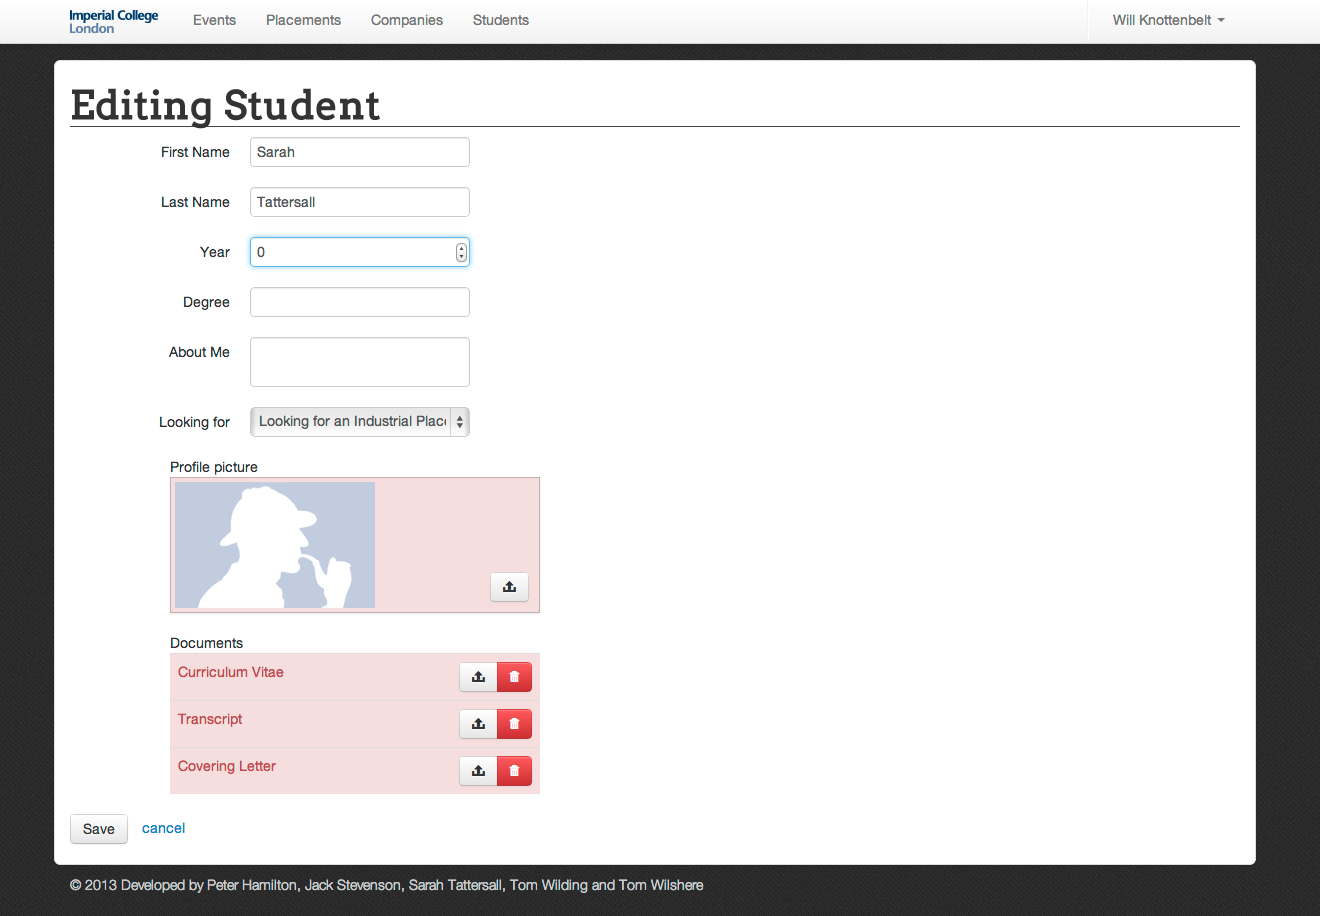
\includegraphics[scale=0.5]{images/user_experiences/admin/admin_student_edit}
    \caption{Student edit page for department administrators.}
    \end{figure}

    On clicking save he is taken to her student view. Will also has the right to be able to delete any students who have either left the department or are causing a problem on the site. We hope the latter will not happen but it is a risk that could happen when students are allowed to develop their own profile.

  \paragraph{Companies:}
    Will can edit, create, and delete companies in exactly the same way as students and can also be directed to a page the edits the companies contacts directly. 

    \begin{figure}[H]\centering
    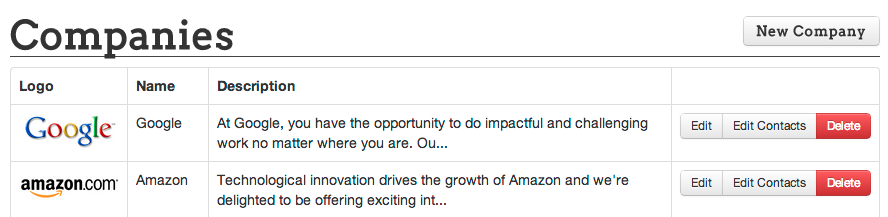
\includegraphics[scale=0.5]{images/user_experiences/admin/admin_company_edit_options}
    \caption{Department admin company edit options.}
    \end{figure}

    The only extra is a company has to be approved by the department administrators in order to have access to students before it will appear in any of their searches.




  \paragraph{Emails:}
